\documentclass[12pt]{article}

% Language setting
\usepackage[utf8]{inputenc}
\usepackage[bulgarian]{babel}

% --------------------- Packages  --------------------
% Use biblatex
\usepackage{biblatex}
\addbibresource{bibliography.bib}
% Table thickness
\usepackage{ctable}
% Equations: SI units
\usepackage{siunitx}
% Approximately equal
\usepackage{amssymb}
% degrees symbol
\usepackage{gensymb}
% warning box
\usepackage{pifont,mdframed}
% Multiple columns
\usepackage{multicol}
% Multiline equation
\usepackage{amsmath}

\newenvironment{warning}
  {\par\begin{mdframed}[linewidth=2pt, linecolor=white]%
    \begin{list}{}{\leftmargin=1cm
                   \labelwidth=\leftmargin}\item[\Large\ding{43}]}
  {\end{list}\end{mdframed}\par}

% --------------------- Title  --------------------
\addbibresource{bibliography.bib}

\begin{document}

\begin{titlepage}
	\flushleft
% 	\begin{center}
	%{\scshape\Large Werkstoffe III \hspace{2.5cm} Laborbericht \hspace{2.5cm}HS 2022 \par}
	{\scshape\Large Протокол V \hspace{2cm} Молекулна физика\par}
	\vspace{4cm}
	{\huge\bfseries Измерване на отношението $C_P/C_V$ на газове по метода на Клемент и Дезорм\par}
	\vspace{1cm}
	{\LARGE\bfseries Лабораторно упражнение №3.4\par}
	\vspace{5cm}
    {\LARGE\bfseries Виолета Кабаджова, \par}
%   {\LARGE\bfseries Group: X\par}
    {\large\bfseries ККТФ, фак. номер: 3PH0600026\par}
	\vspace{1cm}
	
	{\large Физически Факултет, 
	
	Софийски Университет "Св. Климент Охридски"
	
	4 април 2023 г.\par}
	
\end{titlepage}

% \begin{multicols}{2}

\section{Теоритична част}\label{sec:theoretical-part}
Отношението на обмененото от една термодинамична система безкрайно количество топлина $\delta Q$ към съответното изменение на $dT$ на температурата ѝ дефинира физичната величина топлинен капацитет на системата $C^* = \frac{\delta Q}{dT}$. Стойностите ѝ варират между отделните термодинамични процеси, но за конкретен термодинамичен процес остават постоянни. Следователно дефинираме топлинен капацитет при постоянно налягане $C^*_P$ и при постоянен обем $C^*_V$. От първи принцип на динамиката следва уравнение \ref{eq:c-star}.

\begin{equation}\label{eq:c-star}
    C^* = \frac{\delta Q}{dT} = \frac{dU}{dT} + \frac{\delta A}{dT}
\end{equation}

От тази връзка могат да се изразят моларните топлинни капацитети в зависимост от протичащите термодинамични изопроцеси. За изохорен процес, при който $V = const$, $dV = 0$, $\delta A = pdV = 0$, следва уравнение \ref{eq:c-isochoric} (т.е. цялото обменено от газа количество топлина отива за изменение на вътрешната му енергия). За изобарен процес, при който $p = const$, $dp = 0$, взимайки в предвид уравнението за състоянието на един mol идеален газ (ур. \ref{eq:eq-of-states}), следва уравнение \ref{eq:c-isobaric}. За адиабатен процес, при който $\delta Q = 0$, следва, че системата може да извършва работа само за сметка на вътрешната си енергия $\delta A = -dU$ и $C = 0$, откъдето следва уравнението на Поасон (\ref{eq:poisson}), което в $(p, T)$ равнината придобва вида $p^{1-\gamma}T^\gamma = const$ или още може да се запише под формата на ур. \ref{eq:poisson-pt}. Оттук т.нар. коефициент на Поасон (\ref{eq:poisson-gamma}), който ще изследваме в настоящата задача.
% $\frac{T^\gamma}{p^{\gamma - 1}} = const$.

\begin{equation}\label{eq:c-isochoric}
    \left[ \frac{\delta Q}{dT} \right]_V = C_V = \frac{dU}{dT}
\end{equation}

\begin{equation}\label{eq:eq-of-states}
    pV = RT
\end{equation}

\begin{equation}\label{eq:c-isobaric}
    \left[ \frac{\delta Q}{dT} \right]_P = C_P = \frac{dU}{dT} + \frac{\delta A}{dT} = C_V + \frac{pdV}{dT}
\end{equation}

\begin{equation}\label{eq:poisson}
    pV^\gamma = const
\end{equation}

\begin{equation}\label{eq:poisson-pt}
    \frac{T^\gamma}{p^{\gamma - 1}} = const
\end{equation}

\begin{equation}\label{eq:poisson-gamma}
    \gamma = \frac{C_P}{C_V}
\end{equation}

\section{Експериментална част}

\subsection{Експериментална установка}\label{sec:Setup}
\begin{figure}
    \centering
    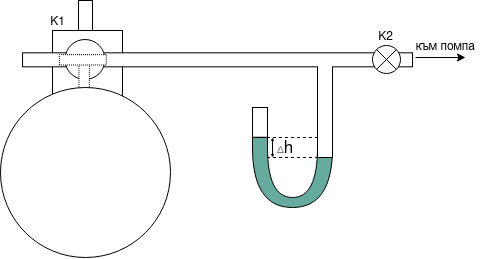
\includegraphics[width=0.8\textwidth]{images/setup.drawio.png}
    \caption{Експериментална установка}
    \label{fig:setup}
\end{figure}

На фиг. \ref{fig:setup} е представена схема на опитната постановка, включваща стъклен балон, U-виден манометър и помпа, свързани чрез система от стъклени тръби. Термодинамичните състояния, през които преминава системата са следните:
\begin{itemize}
    \item Започва се със затворени кранове К1 и К2 (поставен както на схемата). Газът в балона е с налягане и температура еднакви с тази на околната среда ($p_0$, $T_0$). Обемът $V_0$ се определя от обема на системата от балон и тръбитчки до К2, както и от течността в манометъра. 
    \item Адиабатно свиване. При отворен кран К2 и затворен кран К1 бързо се вкарва въздух чрез помпата и кран К1 се затваря. Това предизвиква адиабатен процес, тъй като системата няма време да осъществи ефективен топлообмен с околната среда. Налягането $p_1 = p_0 + \Delta p$ нараства, откъдето в следствие на ур. \ref{eq:eq-of-states} нараства и температурата $T_1 > T_0$
    \item Измерване на $\Delta h_1$ при квазиизохорен процес. При затворени кранове К1 и К2, газта в стъклената система от тръбички и балон започва да обменя топлина с околната среда. В следствие на това температурата започва да спада до $T_0$, откъдето и налягането в балона се понижава до $p_2 = p_0 + \Delta p_1$ ($p_0 < p_2 < p_1$). В този момент нивото на течността в манометъра се променя и отчитаме $\Delta h_1$.
    \item Адиабатно разширяване. За кратко отваряме кран К1, с което свързваме балона с околната среда. По този начин осъществяваме адиабатно разширяване на газта, преминавайки от състояние ($p_2$, $T_0$) до ($p_0$, $T_2$), където $T_2 < T_0$. От уравнение \ref{eq:poisson} следва уравнение \ref{eq:poisson-to-gamma}.

    \begin{equation}\label{eq:poisson-to-gamma}
        \frac{T_0^\gamma}{p_1^{\gamma-1}} = \frac{T_2^\gamma}{p_0^{\gamma-1}}
    \end{equation}
    
    \item Измерване на $\Delta h_2$ при квазиизохорен процес. При затворени кранове К1 и К2 поради топлообмен с околната среда газът се загрява до температура $T_0$ и преминава от състояние ($p_0$, $T_2$) до ($p_2$, $T_0$), където $p_2 = p_0 + \Delta p_2$. Оттук и от уравнение \ref{eq:poisson-to-gamma} следват уравнения \ref{eq:p-over-T} и \ref{eq:p-gammas}.

    \begin{equation}\label{eq:p-over-T}
        \frac{p_0}{T_2} = \frac{p_2}{T_0}
    \end{equation}
    
    \begin{equation}\label{eq:p-gammas}
        p_1^{\gamma - 1}\cdot p_0^\gamma = p_2^\gamma \cdot p_0^{\gamma-1}
    \end{equation}
\end{itemize}

От \ref{eq:p-gammas} и $p_1 = p_0 + \Delta p_1$, $p_2 = p_0 + \Delta p_2$ може да се изведе формула \ref{eq:work-formula}, откъдето посредством формулата за хидростатично налягане следват $\Delta p_1 = \rho_T g \Delta h_1$, $\Delta p_2 = \rho_T g \Delta h_2$ и работната ни формула \ref{eq:work-formula-2}.
    
\begin{equation}\label{eq:work-formula}
    \gamma = \frac{\Delta p_1}{\Delta p_1 - \Delta p_2}
\end{equation}

\begin{equation}\label{eq:work-formula-2}
    \gamma = \frac{C_P}{C_V} = \frac{\Delta h_1}{\Delta h_1 - \Delta h_2}
\end{equation}

\subsection{Задача: Определяне на съотношението $\gamma = \frac{C_P}{C_V}$}
Възпроизвеждаме многократно последователността от процеси, описани в \ref{sec:Setup}, като на записваме стойностите на $\Delta h_1$ и $\Delta h_2$ в таблица \ref{tbl:results} и изчисляваме $\gamma$ за всяка двойка стойности. Извеждаме формулата за абсолютна грешка по начинът, посочен по-долу, като отчитаме, че $\Delta \Delta h_1 = (\Delta_{ins})_{h1} = (\Delta_{ins})_{h2} = \Delta \Delta h_2 = \Delta h$:

\begin{align*}\label{eq:derivation-abs-err}
    \Delta \left[\frac{\Delta h_1}{\Delta h_2 - \Delta h_1}\right] = 
    \frac{\Delta h_1 \Delta [\Delta h_2 - \Delta h_1] + (\Delta h_2 - \Delta h_1)\Delta\Delta h_1}{(\Delta h_2 - \Delta h_1)^2} = \\ 
    = \frac{\Delta h_1 (\Delta\Delta h_2 + \Delta\Delta h_1) + (\Delta h_2 - \Delta h_1)\Delta\Delta h_1}{(\Delta h_2 - \Delta h_1)^2} = \\
    = \frac{\Delta h_1 (2\Delta h) + (\Delta h_2 - \Delta h_1)\Delta h}{(\Delta h_2 - \Delta h_1)^2} = \frac{\Delta h(2\Delta h_1 + \Delta h_2 - \Delta h_1)}{(\Delta h_2 - \Delta h_1)^2} = \\
    = \frac{\Delta h(\Delta h_2 + \Delta h_1)}{(\Delta h_2 - \Delta h_1)^2}
\end{align*}

\begin{table}[h]
\begin{center}
\begin{tabular}{|l|l|l|l|} \hline
        N & \Delta h_1, [cm] & \Delta h_2, [cm] & \gamma_i \\ \hline
        1 & 11.5 & 2.9 & 1.34 \pm 0.02 \\ \hline
        2 & 9.2 & 2.4 & 1.35 \pm 0.03  \\ \hline
        3 & 11.3 & 2.9 & 1.35 \pm 0.02 \\ \hline
        4 & 10.2 & 2.5 & 1.33 \pm 0.02 \\ \hline
        5 & 11.3 & 2.9 & 1.35 \pm 0.02 \\ \hline
        6 & 10.3 & 2.5 & 1.32 \pm 0.02 \\ \hline
        7 & 8.8 & 2.1 & 1.31 \pm 0.2   \\ \hline
        8 & 9.1 & 2.3 & 1.34 \pm 0.03  \\ \hline
        9 & 10.4 & 2.7 & 1.35 \pm 0.02 \\ \hline
        10 & 11.6 & 2.9 & 1.33 \pm 0.02\\ \hline
        
\end{tabular}
\caption{\label{tbl:results}Измервания}
\end{center}
\end{table}

Получаваме, че $\bar{\gamma} = 1.34 \pm 0.01$, като средна стойност на изчислените в таблицата, а грешката отчитаме като сумартната квадратична грешка $\Delta \gamma = \sqrt{\sigma^2 + \Delta_{ins}^2} = \sqrt{\frac{\Sigma^n_{i=1}(\gamma_i - \bar{\gamma})^2}{n-1} + \Delta_{ins}^2}$
% \end{multicols}
\end{document}
